\documentclass[border=8pt]{standalone}
\usepackage[T1]{fontenc}\usepackage{helvet}\renewcommand{\familydefault}{\sfdefault}
\usepackage{tikz}\usetikzlibrary{arrows.meta, positioning, calc, backgrounds}
\definecolor{ink}{HTML}{1a1916}
\definecolor{inktwo}{HTML}{3a3a35}
\definecolor{inkthree}{HTML}{6a6862}
\definecolor{rule}{HTML}{b8b09a}
\definecolor{amber}{HTML}{a8730a}
\definecolor{red}{HTML}{c8261a}
\definecolor{paper}{HTML}{f0eee5}
\definecolor{slab}{HTML}{d8d4c6}
\tikzset{
  >={Stealth[length=2.2mm]},
  wire/.style={line width=0.8pt, ink},
  modwire/.style={line width=0.6pt, dashed, ink},
  tastewire/.style={line width=0.6pt, dashed, amber},
  gatewire/.style={line width=0.6pt, dotted, ink},
  block/.style={rectangle, draw=ink, line width=0.9pt, fill=slab, minimum width=3.0cm, minimum height=1.9cm, inner sep=0pt},
  perf/.style={rectangle, draw=ink, line width=0.7pt, minimum width=3.0cm, minimum height=0.7cm, inner sep=2pt, font=\footnotesize, text=ink},
  title/.style={font=\scriptsize\bfseries, text=ink, anchor=north, inner sep=2pt},
  jack/.style={circle, draw=ink, fill=paper, line width=0.5pt, minimum size=3.2pt, inner sep=0pt},
  plabel/.style={font=\tiny, text=inktwo, anchor=west, inner sep=1pt},
  olabel/.style={font=\tiny, text=inktwo, anchor=east, inner sep=1pt},
  settings/.style={font=\scriptsize, text=ink, align=left, anchor=north west, inner sep=1pt, text width=2.9cm},
}
\begin{document}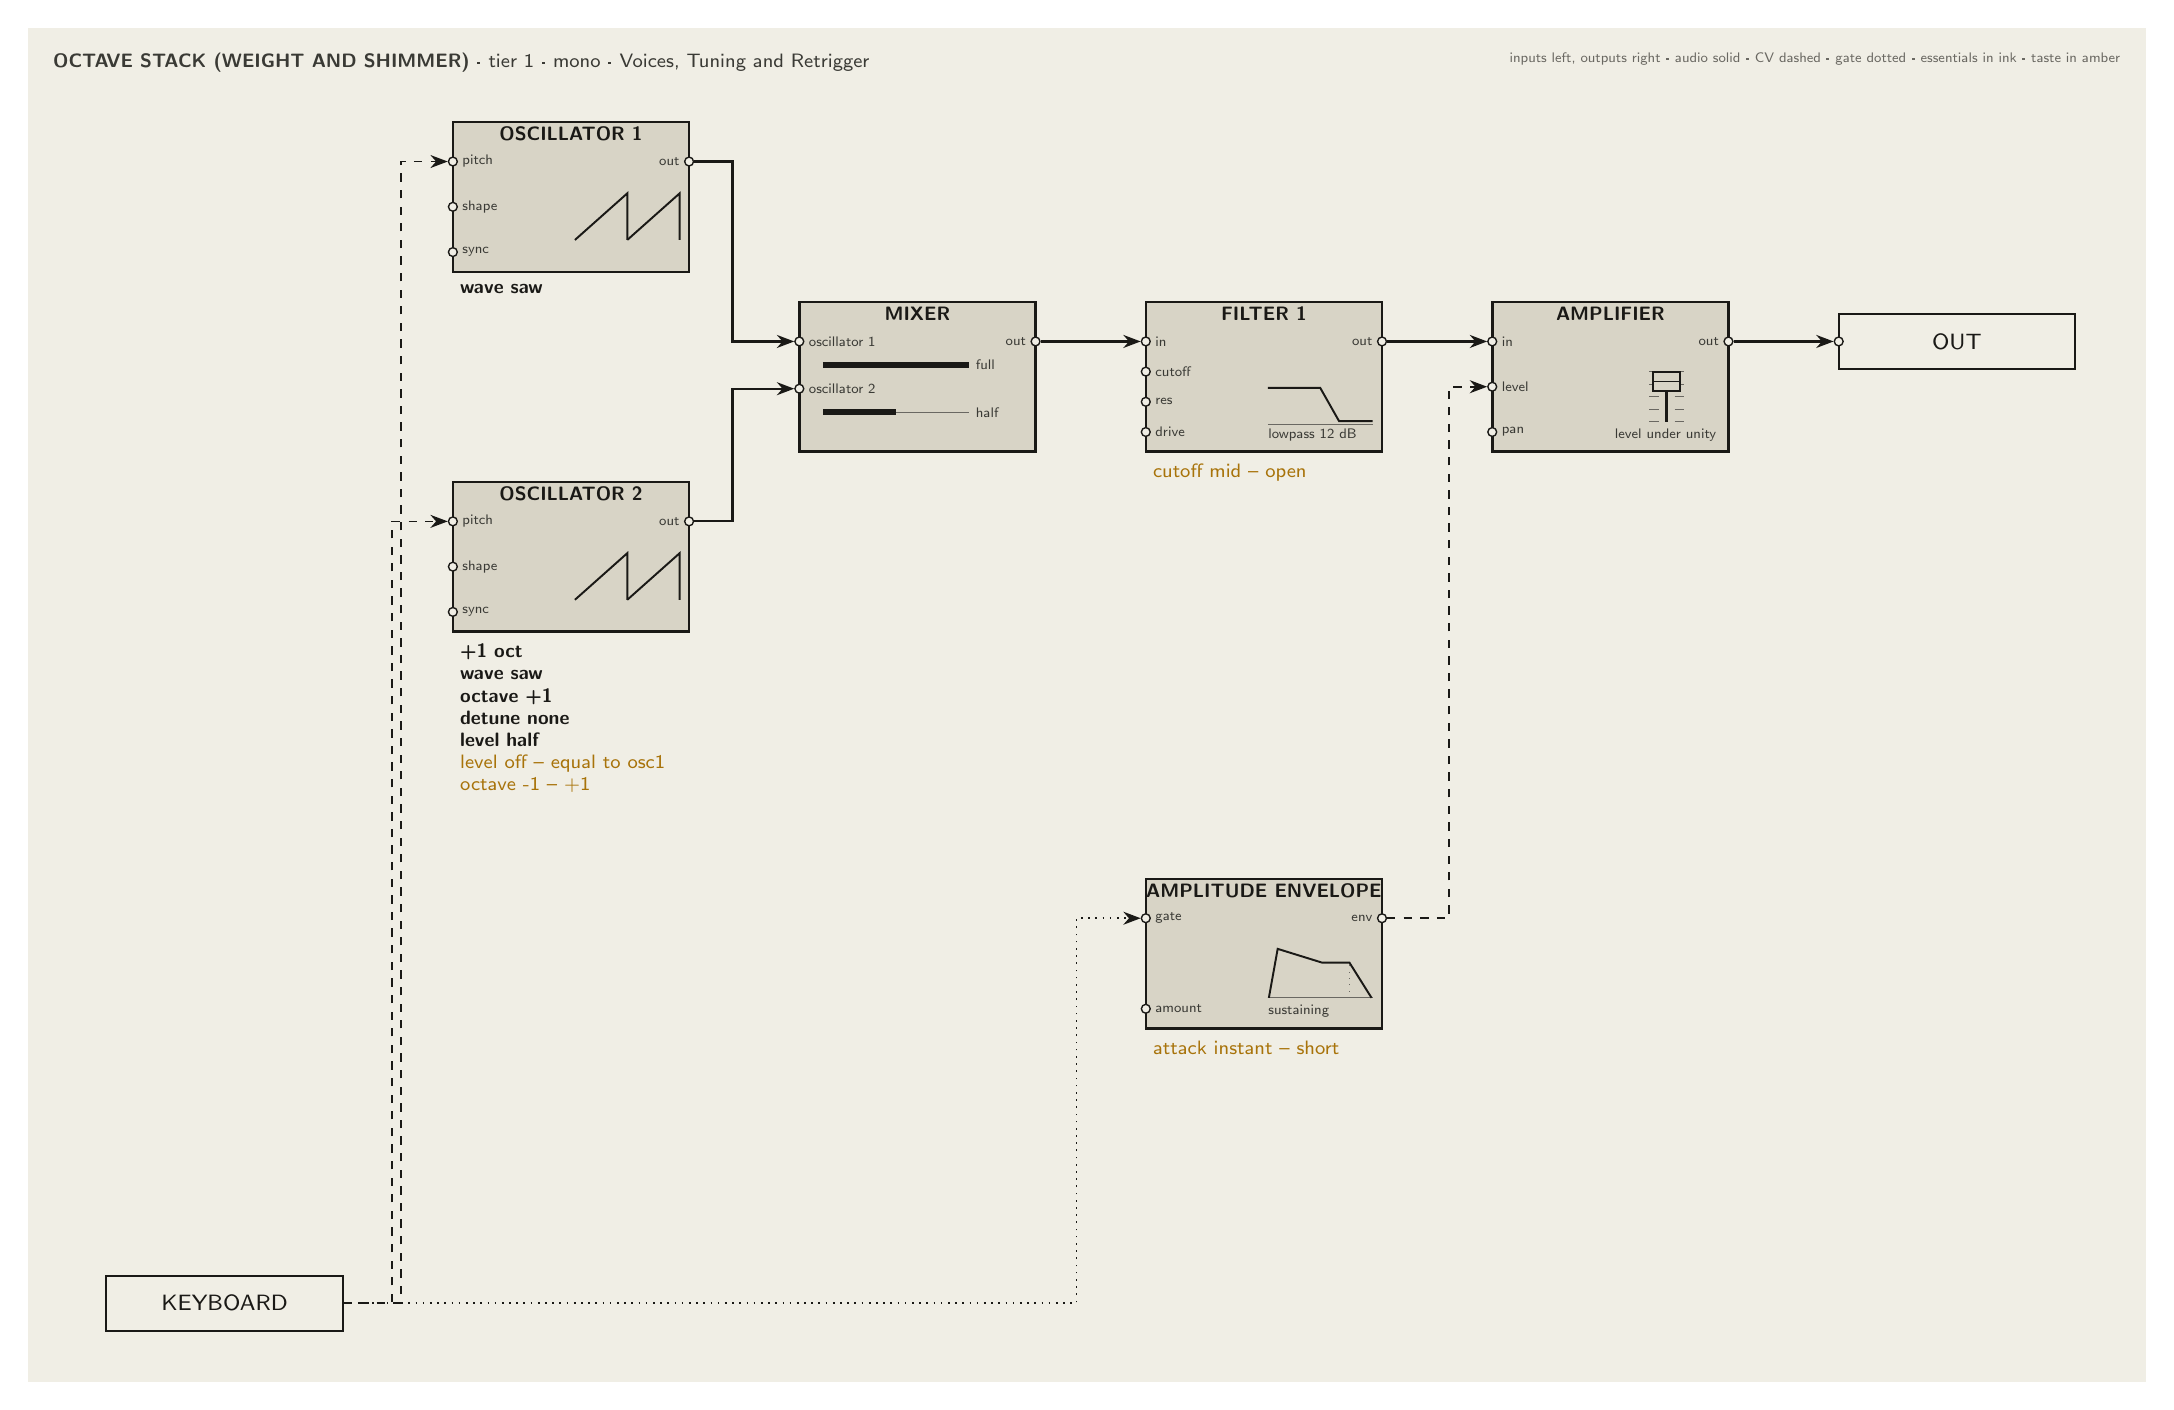
\begin{tikzpicture}
\begin{scope}[on background layer]\fill[paper] (-2.5,-12.764999999999999) rectangle (24.4,4.4350000000000005);\end{scope}
\node[block, minimum height=1.9cm] (osc1) at (4.4,2.285) {};
\node[title] at (osc1.north) {OSCILLATOR 1};
\node[jack] (osc1-pitch) at (2.9000000000000004,2.7350000000000003) {};
\node[plabel] at (2.9800000000000004,2.7350000000000003) {pitch};
\node[jack] (osc1-shape) at (2.9000000000000004,2.16) {};
\node[plabel] at (2.9800000000000004,2.16) {shape};
\node[jack] (osc1-sync) at (2.9000000000000004,1.5850000000000004) {};
\node[plabel] at (2.9800000000000004,1.5850000000000004) {sync};
\node[jack] (osc1-out) at (5.9,2.7350000000000003) {};
\node[olabel] at (5.82,2.7350000000000003) {out};
\begin{scope}
\draw[ink, line width=0.7pt] (4.450,1.739) -- (5.115,2.331) -- (5.115,1.739);
\draw[ink, line width=0.7pt] (5.115,1.739) -- (5.780,2.331) -- (5.780,1.739);
\end{scope}
\node[settings] at (2.95,1.2150000000000003) {\textbf{wave saw}};
\node[block, minimum height=1.9cm] (osc2) at (4.4,-2.285) {};
\node[title] at (osc2.north) {OSCILLATOR 2};
\node[jack] (osc2-pitch) at (2.9000000000000004,-1.8350000000000002) {};
\node[plabel] at (2.9800000000000004,-1.8350000000000002) {pitch};
\node[jack] (osc2-shape) at (2.9000000000000004,-2.41) {};
\node[plabel] at (2.9800000000000004,-2.41) {shape};
\node[jack] (osc2-sync) at (2.9000000000000004,-2.9850000000000003) {};
\node[plabel] at (2.9800000000000004,-2.9850000000000003) {sync};
\node[jack] (osc2-out) at (5.9,-1.8350000000000002) {};
\node[olabel] at (5.82,-1.8350000000000002) {out};
\begin{scope}
\draw[ink, line width=0.7pt] (4.450,-2.831) -- (5.115,-2.239) -- (5.115,-2.831);
\draw[ink, line width=0.7pt] (5.115,-2.831) -- (5.780,-2.239) -- (5.780,-2.831);
\end{scope}
\node[settings] at (2.95,-3.3550000000000004) {\textbf{+1 oct} \\ \textbf{wave saw} \\ \textbf{octave +1} \\ \textbf{detune none} \\ \textbf{level half} \\ \textcolor{amber}{level off -- equal to osc1} \\ \textcolor{amber}{octave -1 -- +1}};
\node[block, minimum height=1.9cm] (mix) at (8.8,0.0) {};
\node[title] at (mix.north) {MIXER};
\node[jack] (mix-osc1) at (7.300000000000001,0.44999999999999996) {};
\node[plabel] at (7.380000000000001,0.44999999999999996) {oscillator 1};
\draw[inkthree, line width=0.3pt] (7.600,0.150) -- (9.450,0.150);
\draw[ink, line width=2.2pt] (7.600,0.150) -- (9.450,0.150);
\node[font=\tiny, text=inktwo, anchor=west, inner sep=1pt] at (9.500,0.150) {full};
\node[jack] (mix-osc2) at (7.300000000000001,-0.15000000000000002) {};
\node[plabel] at (7.380000000000001,-0.15000000000000002) {oscillator 2};
\draw[inkthree, line width=0.3pt] (7.600,-0.450) -- (9.450,-0.450);
\draw[ink, line width=2.2pt] (7.600,-0.450) -- (8.525,-0.450);
\node[font=\tiny, text=inktwo, anchor=west, inner sep=1pt] at (9.500,-0.450) {half};
\node[jack] (mix-out) at (10.3,0.44999999999999996) {};
\node[olabel] at (10.22,0.44999999999999996) {out};
\node[block, minimum height=1.9cm] (filter1) at (13.200000000000001,0.0) {};
\node[title] at (filter1.north) {FILTER 1};
\node[jack] (filter1-in) at (11.700000000000001,0.44999999999999996) {};
\node[plabel] at (11.780000000000001,0.44999999999999996) {in};
\node[jack] (filter1-cutoff) at (11.700000000000001,0.06666666666666665) {};
\node[plabel] at (11.780000000000001,0.06666666666666665) {cutoff};
\node[jack] (filter1-res) at (11.700000000000001,-0.31666666666666665) {};
\node[plabel] at (11.780000000000001,-0.31666666666666665) {res};
\node[jack] (filter1-drive) at (11.700000000000001,-0.7) {};
\node[plabel] at (11.780000000000001,-0.7) {drive};
\node[jack] (filter1-out) at (14.700000000000001,0.44999999999999996) {};
\node[olabel] at (14.620000000000001,0.44999999999999996) {out};
\begin{scope}
\draw[inkthree, line width=0.3pt] (13.250,-0.605) -- (14.580,-0.605);
\draw[ink, line width=0.7pt] (13.250,-0.139) -- (13.915,-0.139) -- (14.154,-0.561) -- (14.580,-0.561);
\node[font=\tiny, text=inktwo, anchor=north west, inner sep=0pt] at (13.250,-0.650) {lowpass 12 dB};
\end{scope}
\node[settings] at (11.750000000000002,-1.0699999999999998) {\textcolor{amber}{cutoff mid -- open}};
\node[block, minimum height=1.9cm] (amp) at (17.6,0.0) {};
\node[title] at (amp.north) {AMPLIFIER};
\node[jack] (amp-in) at (16.1,0.44999999999999996) {};
\node[plabel] at (16.18,0.44999999999999996) {in};
\node[jack] (amp-level) at (16.1,-0.125) {};
\node[plabel] at (16.18,-0.125) {level};
\node[jack] (amp-pan) at (16.1,-0.7) {};
\node[plabel] at (16.18,-0.7) {pan};
\node[jack] (amp-out) at (19.1,0.44999999999999996) {};
\node[olabel] at (19.020000000000003,0.44999999999999996) {out};
\begin{scope}
\draw[ink, line width=1.2pt] (18.315,-0.570) -- (18.315,0.070);
\draw[inkthree, line width=0.3pt] (18.095,-0.570) -- (18.215,-0.570) (18.415,-0.570) -- (18.535,-0.570);
\draw[inkthree, line width=0.3pt] (18.095,-0.410) -- (18.215,-0.410) (18.415,-0.410) -- (18.535,-0.410);
\draw[inkthree, line width=0.3pt] (18.095,-0.250) -- (18.215,-0.250) (18.415,-0.250) -- (18.535,-0.250);
\draw[inkthree, line width=0.3pt] (18.095,-0.090) -- (18.215,-0.090) (18.415,-0.090) -- (18.535,-0.090);
\draw[inkthree, line width=0.3pt] (18.095,0.070) -- (18.215,0.070) (18.415,0.070) -- (18.535,0.070);
\fill[slab, draw=ink, line width=0.6pt] (18.145,-0.178) rectangle (18.485,0.062);
\draw[ink, line width=0.5pt] (18.145,-0.058) -- (18.485,-0.058);
\node[font=\tiny, text=inktwo, anchor=north west, inner sep=0pt] at (17.650,-0.650) {level under unity};
\end{scope}
\node[block, minimum height=1.9cm] (aenv) at (13.200000000000001,-7.325000000000001) {};
\node[title] at (aenv.north) {AMPLITUDE ENVELOPE};
\node[jack] (aenv-gate) at (11.700000000000001,-6.875000000000001) {};
\node[plabel] at (11.780000000000001,-6.875000000000001) {gate};
\node[jack] (aenv-amount) at (11.700000000000001,-8.025) {};
\node[plabel] at (11.780000000000001,-8.025) {amount};
\node[jack] (aenv-out) at (14.700000000000001,-6.875000000000001) {};
\node[olabel] at (14.620000000000001,-6.875000000000001) {env};
\begin{scope}
\draw[inkthree, line width=0.3pt] (13.250,-7.886) -- (14.580,-7.886);
\draw[ink, line width=0.7pt] (13.263,-7.886) -- (13.375,-7.264) -- (13.936,-7.438) -- (14.286,-7.438) -- (14.567,-7.886);
\draw[inkthree, line width=0.3pt, dotted] (14.286,-7.886) -- (14.286,-7.438);
\node[font=\tiny, text=inktwo, anchor=north west, inner sep=0pt] at (13.250,-7.975) {sustaining};
\end{scope}
\node[settings] at (11.750000000000002,-8.395) {\textcolor{amber}{attack instant -- short}};
\node[perf] (key) at (0.0,-11.764999999999999) {KEYBOARD};
\node[perf, fill=paper] (out) at (22.0,0.44999999999999996) {OUT}; \node[jack] (out-in) at (20.5,0.44999999999999996) {};
\draw[wire,->] (osc1-out) -- (6.45,2.7350000000000003) |- (mix-osc1);
\draw[wire,->] (osc2-out) -- (6.45,-1.8350000000000002) |- (mix-osc2);
\draw[wire,->] (mix-out) -- (filter1-in);
\draw[wire,->] (filter1-out) -- (amp-in);
\draw[wire,->] (amp-out) -- (out-in);
\draw[modwire,->] (aenv-out) -- (15.55,-6.875000000000001) -- (15.55,-0.125) -- (amp-level);
\draw[modwire,->] (key.east) -- (2.2400000000000007,-11.764999999999999) -- (2.2400000000000007,2.7350000000000003) -- (osc1-pitch);
\draw[modwire,->] (key.east) -- (2.1300000000000003,-11.764999999999999) -- (2.1300000000000003,-1.8350000000000002) -- (osc2-pitch);
\draw[gatewire,->] (key.east) -- (10.82,-11.764999999999999) -- (10.82,-6.875000000000001) -- (aenv-gate);
\node[anchor=north west, font=\scriptsize, text=inktwo] at (-2.3,4.235) {\textbf{OCTAVE STACK (WEIGHT AND SHIMMER)} · tier 1 · mono · Voices, Tuning and Retrigger};
\node[anchor=north east, font=\tiny, text=inkthree] at (24.2,4.235) {inputs left, outputs right · audio solid · CV dashed · gate dotted · essentials in ink · taste in amber};
\end{tikzpicture}\end{document}
